\section{Requirements}

\subsection{External Interface Requirements}

\begin{figure}[h!]
    \centering
    \scalebox{0.85}{
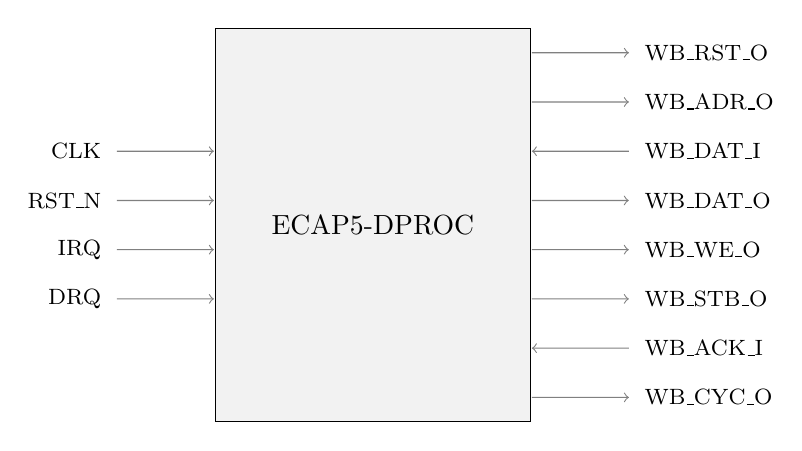
\begin{tikzpicture}[scale=1.25, draw=gray, inner sep=0, outer sep=0]
  \node[rectangle, draw=black,
    minimum height = 5cm,
    minimum width = 4cm,
    fill = gray!10] (box) at (0, 0) {ECAP5-DPROC};

  % left
  \node (lport1) at ([yshift=0.75cm]box.west) {};
  \node (lport2) at ([yshift=0.25cm]box.west) {};
  \node (lport3) at ([yshift=-0.25cm]box.west) {};
  \node (lport4) at ([yshift=-0.75cm]box.west) {};

  \draw[->] ([xshift=-1cm]lport1.center) node[left=0.2cm, anchor=east]{\footnotesize CLK} -- (lport1);
  \draw[->] ([xshift=-1cm]lport2.center) node[left=0.2cm, anchor=east]{\footnotesize RST\_N} -- (lport2);
  \draw[->] ([xshift=-1cm]lport3.center) node[left=0.2cm, anchor=east]{\footnotesize IRQ} -- (lport3);
  \draw[->] ([xshift=-1cm]lport4.center) node[left=0.2cm, anchor=east]{\footnotesize DRQ} -- (lport4);

  % right
  \node (rport4) at ([yshift=0.25cm]box.east) {};
  \node (rport3) at ([yshift=0.5cm]rport4.center) {};
  \node (rport2) at ([yshift=0.5cm]rport3.center) {};
  \node (rport1) at ([yshift=0.5cm]rport2.center) {};

  \node (rport5) at ([yshift=-0.25cm]box.east) {};
  \node (rport6) at ([yshift=-0.5cm]rport5.center) {};
  \node (rport7) at ([yshift=-0.5cm]rport6.center) {};
  \node (rport8) at ([yshift=-0.5cm]rport7.center) {};

  \draw[<-] ([xshift=1cm]rport1.center) node[right=0.2cm, anchor=west]{\footnotesize WB\_RST\_O} -- (rport1);
  \draw[<-] ([xshift=1cm]rport2.center) node[right=0.2cm, anchor=west]{\footnotesize WB\_ADR\_O} -- (rport2);
  \draw[->] ([xshift=1cm]rport3.center) node[right=0.2cm, anchor=west]{\footnotesize WB\_DAT\_I} -- (rport3);
  \draw[<-] ([xshift=1cm]rport4.center) node[right=0.2cm, anchor=west]{\footnotesize WB\_DAT\_O} -- (rport4);
  \draw[<-] ([xshift=1cm]rport5.center) node[right=0.2cm, anchor=west]{\footnotesize WB\_WE\_O} -- (rport5);
  \draw[<-] ([xshift=1cm]rport6.center) node[right=0.2cm, anchor=west]{\footnotesize WB\_STB\_O} -- (rport6);
  \draw[->] ([xshift=1cm]rport7.center) node[right=0.2cm, anchor=west]{\footnotesize WB\_ACK\_I} -- (rport7);
  \draw[<-] ([xshift=1cm]rport8.center) node[right=0.2cm, anchor=west]{\footnotesize WB\_CYC\_O} -- (rport8);
\end{tikzpicture}
}

    \caption{Schematic view of the external interface of ECAP5-DPROC}
    \label{fig:externalinterface}
\end{figure}

\begin{table}[H]
  \centering
  {
\footnotesize
\begin{tabularx}{0.9\textwidth}{|l|c|c|X|}
  \hline
  \cellcolor{gray!20}\textbf{NAME} & \cellcolor{gray!20}\textbf{TYPE} & \cellcolor{gray!20}\textbf{WIDTH} & \cellcolor{gray!20}\textbf{DESCRIPTION} \\
  \hline
  CLK & I & 1 & Clock input. \\
  \hline
  RST\_N & I & 1 & Hardware reset. Active low. \\
  \hline
  IRQ & I & 1 & External interrupt request. \\
  \hline
  DRQ & I & 1 & Debug request. \\
  \hline
\end{tabularx}
}

  \caption{ECAP5-DPROC control signals}
  \label{tab:control-interface}
\end{table}

\begin{table}[H]
  \centering
  {
\footnotesize
\begin{tabularx}{0.9\textwidth}{|l|c|c|X|}
  \hline
  \cellcolor{gray!20}\textbf{NAME} & \cellcolor{gray!20}\textbf{TYPE} & \cellcolor{gray!20}\textbf{WIDTH} & \cellcolor{gray!20}\textbf{DESCRIPTION} \\
  \hline
  \multicolumn{4}{|l|}{\textbf{READ ADDRESS BUS}} \\
  \hline
  ARADDR & O & 32 & Read address. \\
  \hline
  ARVALID & O & 1 & Read address valid. \\
  \hline
  ARREADY & I & 1 & Read address ready. \\ 
  \hline
  \multicolumn{4}{|l|}{\textbf{READ DATA BUS}} \\
  \hline
  RDATA & I & 32 & Read data. \\
  \hline
  RRESP & I & 2 & Read response. \\
  \hline
  RVALID & I & 1 & Read valid. \\
  \hline
  RREADY & O & 1 & Read ready. \\ 
  \hline
  \multicolumn{4}{|l|}{\textbf{WRITE ADDRESS BUS}} \\
  \hline
  AWADDR & O & 32 & Write address. \\
  \hline
  AWVALID & O & 1 & Write address valid. \\
  \hline
  AWREADY & I & 1 & Write address ready \\
  \hline
  \multicolumn{4}{|l|}{\textbf{WRITE DATA BUS}} \\
  \hline
  WDATA & O & 32 & Write data. \\
  \hline
  WSTRB & O & 4 & Write strobes. \\
  \hline
  \multicolumn{4}{|l|}{\textbf{WRITE RESPONSE BUS}} \\
  \hline
  BRESP & I & 2 & Write response. \\
  \hline
  BVALID & I & 1 & Write response valid. \\
  \hline
  BREADY & O & 1 & Response ready. \\
  \hline
\end{tabularx}
}

  \caption{ECAP5-DPROC memory interface signals}
  \label{tab:memory-interface}
\end{table}

\req{I\_CLK\_01}{
  All inputs and outputs of ECAP5-DPROC shall belong to CLK's clock domain.
}

\req{I\_RESET\_01}{
  The RST\_N signal shall hold ECAP5-DPROC in a reset state while asserted.
}[
  derivedfrom=U\_RESET\_01
]

\req{I\_RESET\_02}{
  RST\_N polarity shall be active low.
}

\req{I\_IRQ\_01}{
  ECAP5-DPROC shall jump to a software-configurable address when input IRQ is asserted.
}[
  derivedfrom={U\_HARDWARE\_INTERRUPT\_01, U\_HARDWARE\_INTERRUPT\_02}
]

\req{I\_DIRQ\_01}{
  TBC
}

\req{I\_MEMORY\_INTERFACE\_01}{
  Signals from table \ref{tab:memory-interface} shall be compliant with the Wishbone specification.
}[
  derivedfrom=U\_MEMORY\_INTERFACE\_02
]

\begin{content}
  Behavioral specification for symbols in table \ref{tab:memory-interface} is outlined in the functional requirements section, subsection \ref{spec-memory-interface}.
\end{content}

\subsection{Functional Requirements}

\subsubsection{Register file}

\req{F\_REGISTERS\_01}{
  ECAP5-DPROC shall implement 32 user-accessible general purpose registers ranging from \texttt{x0} to \texttt{x31}.
}[
  derivedfrom=U\_INSTRUCTION\_SET\_01
]

\req{F\_REGISTERS\_02}{
  Register \texttt{x0} shall always be equal to zero.
}[
  derivedfrom=U\_INSTRUCTION\_SET\_01
]

\req{F\_REGISTERS\_03}{
  ECAP5-DPROC shall implement a \texttt{pc} register storing the address of the current instruction, user-accessible through the AUIPC instruction.
}[
  derivedfrom=U\_INSTRUCTION\_SET\_01
]

\subsubsection{Instruction decoding}

\begin{content}
  Figure \ref{fig:instructionencoding} outlines the different instruction encodings for the RV32I instruction set. The \texttt{opcode} parameter is a unique identifier for each instruction. The instruction encoding is infered from the opcode as there can only be one encoding per opcode.
\end{content}

\begin{figure}[h!]
    \centering
    \vspace{0.5em}

\hspace{2em}
\scalebox{0.9}{
\begin{bytefield}[
    bitwidth=1.1em, 
    endianness=big, 
    bitformatting={\scriptsize}, 
    boxformatting={\centering\footnotesize\ttfamily},
    rightcurly=., rightcurlyspace=5pt
]{32}
  \bitheader{0,6,7,8,11,12,14,15,19,20,24,25,31} \\
  \begin{rightwordgroup}{\footnotesize R-type}
    \bitbox{7}{funct7}
    \bitbox{5}{rs2}
    \bitbox{5}{rs1}
    \bitbox{3}{func3}
    \bitbox{5}{rd}
    \bitbox{7}{opcode}
  \end{rightwordgroup}
  \\[2ex]
  \begin{rightwordgroup}{\footnotesize I-type}
    \bitbox{12}{imm[11:0]}
    \bitbox{5}{rs1}
    \bitbox{3}{func3}
    \bitbox{5}{rd}
    \bitbox{7}{opcode}
  \end{rightwordgroup}
  \\[2ex]
  \begin{rightwordgroup}{\footnotesize S-type}
    \bitbox{7}{imm[11:5]}
    \bitbox{5}{rs2}
    \bitbox{5}{rs1}
    \bitbox{3}{func3}
    \bitbox{5}{imm[4:0]}
    \bitbox{7}{opcode}
  \end{rightwordgroup}
  \\[2ex]
  \begin{rightwordgroup}{\footnotesize B-type}
    \bitbox{1}{a}
    \bitbox{6}{imm[10:5]}
    \bitbox{5}{rs2}
    \bitbox{5}{rs1}
    \bitbox{3}{func3}
    \bitbox{4}{imm[4:1]}
    \bitbox{1}{b}
    \bitbox{7}{opcode}
  \end{rightwordgroup}
  \\[2ex]
  \begin{rightwordgroup}{\footnotesize U-type}
    \bitbox{20}{imm[31:12]}
    \bitbox{5}{rd}
    \bitbox{7}{opcode}
  \end{rightwordgroup}
  \\[2ex]
  \begin{rightwordgroup}{\footnotesize J-type}
    \bitbox{1}{c}
    \bitbox{10}{imm[10:1]}
    \bitbox{1}{b}
    \bitbox{8}{imm[31:12]}
    \bitbox{5}{rd}
    \bitbox{7}{opcode}
  \end{rightwordgroup}
\end{bytefield}
}

\vspace{0.25em}
\scalebox{0.7}{
\begin{tabularx}{0.8\textwidth}{Y Y Y}
a: \texttt{imm[12]} & b: \texttt{imm[11]} & c: \texttt{imm[20]}
\end{tabularx}
}

    \caption{Instruction encodings of the RV32I instruction set}
    \label{fig:instructionencoding}
\end{figure}

\paragraph{Immediate encoding}

\begin{content}
  Only one immediate value can be encoded in one instruction. The value can be reconstructed from fragments of the following format : imm[x] representing the x\textsuperscript{th} bit or imm[x:y] representing bits from the x\textsuperscript{th} to the y\textsuperscript{th} both included.
\end{content}

\req{F\_INSTR\_IMMEDIATE\_01}{
  Immediate values shall be sign-extended.
}[
  derivedfrom=U\_INSTRUCTION\_SET\_01
]

\req{F\_INSTR\_IMMEDIATE\_02}{
  The value of an instruction immediate shall be the concatenation of immediate fragments from the instruction encoding.
}[
  derivedfrom=U\_INSTRUCTION\_SET\_01
]

\req{F\_INSTR\_IMMEDIATE\_03}{
  Missing immediate fragments shall be replaced by zeros.
}[
  derivedfrom=U\_INSTRUCTION\_SET\_01
]

\begin{content}
  RV32I is called a Load/Store ISA, meaning that instructions inputs and outputs are passed through registers or through an instruction immediate. There are specific instructions for loading and storing data into memory.
\end{content}

\paragraph{Instruction parameters}

\req{F\_INSTR\_FIRST\_PARAM\_01}{
  Instructions encoded using the R-type, I-type, S-type and B-type shall take as their first parameter the value stored in the register designated by the \texttt{rs1} field.
}[
  derivedfrom=U\_INSTRUCTION\_SET\_01
]

\req{F\_INSTR\_FIRST\_PARAM\_02}{
  Instructions encoded using the U-type and J-type shall take as their first parameter the immediate value encoded in the instruction.
}[
  derivedfrom=U\_INSTRUCTION\_SET\_01
]

\req{F\_INSTR\_SECOND\_PARAM\_01}{
  Instructions encoded using the R-type, S-type and B-type shall take as their second parameter the value stored in the register designated by the \texttt{rs2} field.
}[
  derivedfrom=U\_INSTRUCTION\_SET\_01
]

\req{F\_INSTR\_SECOND\_PARAM\_02}{
  Instructions encoded using the I-type shall take as its second parameter the immediate value encoded in the instruction.
}[
  derivedfrom=U\_INSTRUCTION\_SET\_01
]

\req{F\_INSTR\_THIRD\_PARAM\_01}{
  Instructions encoded using the S-type and B-type shall take as their third parameter the immediate value encoded in the instruction.
}[
  derivedfrom=U\_INSTRUCTION\_SET\_01
]

\paragraph{Instruction results}

\req{F\_INSTR\_RESULT\_01}{
  Instructions encoded using the R-type, I-type, U-type and J-type shall store their result in the register designated by the \texttt{rd} field.
}[
  derivedfrom=U\_INSTRUCTION\_SET\_01
]

\req{F\_INSTR\_RESULT\_02}{
  Instructions encoded using the S-type and B-type do not produce any result.
}[
  derivedfrom=U\_INSTRUCTION\_SET\_01
]

\paragraph{Instruction variants}

\req{F\_INSTR\_VARIANT\_01}{
  Instructions encoded using the R-type, I-type, S-type and B-type shall use the \texttt{func3} field as a behavior variant selector.
}[
  derivedfrom=U\_INSTRUCTION\_SET\_01
]

\req{F\_INSTR\_VARIANT\_02}{
  Instructions encoded using the R-type shall use the \texttt{func7} field as a secondary behavior variant selector.
}[
  derivedfrom=U\_INSTRUCTION\_SET\_01
]

\paragraph{Opcodes}

\vspace{1em}
\begin{content}
  Table \ref{tab:opcodemap} outlines the different opcodes values of the RV32I instruction set. Cells marked as \textit{noimp} are for opcodes that are not implemented in ECAP5-DPROC.
\end{content}

\begin{table}[H]
  \centering
  \scalebox{0.8}{
\footnotesize
\begin{tabular}{|r|c|c|c|c|c|c|c|c|}
  \hline
  opcode[1:0] & \multicolumn{8}{|c|}{11} \\
  \hline
  opcode[4:2] & \multirow{2}{*}{000} & \multirow{2}{*}{001} & \multirow{2}{*}{010} & \multirow{2}{*}{011} & \multirow{2}{*}{100} & \multirow{2}{*}{101} & \multirow{2}{*}{110} & \multirow{2}{*}{111} \\
  \cline{1-1}
  opcode[6:5] & & & & & & & & \\
  \hline
  00 & LOAD & \cellcolor{gray!20}\textit{noimp} & \cellcolor{gray!20}\textit{noimp} & MISC-MEM & OP-IMM & AUIPC & \cellcolor{gray!20}\textit{noimp} & \cellcolor{gray!20}\textit{noimp} \\
  \hline
  01 & STORE & \cellcolor{gray!20}\textit{noimp} & \cellcolor{gray!20}\textit{noimp} & \cellcolor{gray!20}\textit{noimp} & OP & LUI & \cellcolor{gray!20}\textit{noimp} & \cellcolor{gray!20}\textit{noimp} \\
  \hline
  10 & \cellcolor{gray!20}\textit{noimp} & \cellcolor{gray!20}\textit{noimp} & \cellcolor{gray!20}\textit{noimp} & \cellcolor{gray!20}\textit{noimp} & \cellcolor{gray!20}\textit{noimp} & \cellcolor{gray!20}\textit{noimp} & \cellcolor{gray!20}\textit{noimp} & \cellcolor{gray!20}\textit{noimp} \\
  \hline
  11 & BRANCH & JALR & \cellcolor{gray!20}\textit{noimp} & JAL & SYSTEM & \cellcolor{gray!20}\textit{noimp} & \cellcolor{gray!20}\textit{noimp} & \cellcolor{gray!20}\textit{noimp} \\
  \hline
\end{tabular}
}

  \caption{Opcode values for the RV32I instruction set.}
  \label{tab:opcodemap}
\end{table}

\req{F\_OPCODE\_ENCODING\_01}{
  Instructions which use the LUI opcode shall be decoded as an U-type instruction.
}[
  derivedfrom=U\_INSTRUCTION\_SET\_01
]

\req{F\_OPCODE\_ENCODING\_02}{
  Instructions which use the AUIPC opcode shall be decoded as an U-type instruction.
}[
  derivedfrom=U\_INSTRUCTION\_SET\_01
]

\req{F\_OPCODE\_ENCODING\_03}{
  Instructions which use the JAL opcode shall be decoded as a J-type instruction.
}[
  derivedfrom=U\_INSTRUCTION\_SET\_01
]


\req{F\_OPCODE\_ENCODING\_04}{
  Instructions which use the JALR opcode shall be decoded as an I-type instruction.
}[
  derivedfrom=U\_INSTRUCTION\_SET\_01
]

\req{F\_OPCODE\_ENCODING\_05}{
  Instructions which use the BRANCH opcode shall be decoded as a B-type instruction.
}[
  derivedfrom=U\_INSTRUCTION\_SET\_01
]

\req{F\_OPCODE\_ENCODING\_06}{
  Instructions which use the LOAD opcode shall be decoded as an I-type instruction.
}[
  derivedfrom=U\_INSTRUCTION\_SET\_01
]

\req{F\_OPCODE\_ENCODING\_07}{
  Instructions which use the STORE opcode shall be decoded as a S-type instruction.
}[
  derivedfrom=U\_INSTRUCTION\_SET\_01
]

\req{F\_OPCODE\_ENCODING\_08}{
  Instructions which use the OP-IMM opcode shall be decoded as an I-type instruction.
}[
  derivedfrom=U\_INSTRUCTION\_SET\_01
]

\req{F\_OPCODE\_ENCODING\_09}{
  Instructions which use the OP opcode shall be decoded as a R-type instruction.
}[
  derivedfrom=U\_INSTRUCTION\_SET\_01
]

\req{F\_OPCODE\_ENCODING\_10}{
  Instructions which use the MISC-MEM opcode shall be decoded as an I-type instruction.
}[
  derivedfrom=U\_INSTRUCTION\_SET\_01
]

\req{F\_OPCODE\_ENCODING\_11}{
  Instructions which use the SYSTEM opcode shall be decoded as an I-type instruction.
}[
  derivedfrom=U\_INSTRUCTION\_SET\_01
]

\subsubsection{Instructions behaviors}

\label{instruction-behaviors-requirements}

\paragraph{LUI}

\req{F\_LUI\_01}{
  The LUI behavior shall be applied when the opcode is LUI.
}[
  derivedfrom=U\_INSTRUCTION\_SET\_01
]

\req{F\_ADDI\_02}{
  The result of LUI shall be the value of its first parameter.
}[
  derivedfrom=U\_INSTRUCTION\_SET\_01,
  rationale=The LUI instruction shall load the 20 upper bits of the instruction immediate into the destination register and fill the remaining bits with zeros. This is the default behavior for instruction immediates as stated in F\_INSTR\_IMMEDIATE\_02 and F\_INSTR\_IMMEDIATE\_03.
]

\paragraph{AUIPC}

\req{F\_AUIPC\_01}{
  The AUIPC behavior shall be applied when the opcode is AUIPC.
}[
  derivedfrom=U\_INSTRUCTION\_SET\_01
]

\req{F\_AUIPC\_02}{
  The result of AUIPC shall be the sum of its first parameter and the address of the AUIPC instruction.
}[
  derivedfrom=U\_INSTRUCTION\_SET\_01
]

\paragraph{JAL}

\req{F\_JAL\_01}{
  The JAL behavior shall be applied when the opcode is JAL.
}[
  derivedfrom=U\_INSTRUCTION\_SET\_01
]

\req{F\_JAL\_02}{
  The \texttt{pc} register shall be updated with the sum of the address of the JAL instruction with the first instruction parameter. 
}[
  derivedfrom=U\_INSTRUCTION\_SET\_01
]

\req{F\_JAL\_03}{
  The result of JAL shall be the address of the JAL instruction incremented by 4.
}[
  derivedfrom=U\_INSTRUCTION\_SET\_01,
  rationale=The JAL instruction shall output the address to the following instruction for it to be used as a \textit{return address} in the case of a function call.
]

\paragraph{JALR}

\req{F\_JALR\_01}{
  The JALR behavior shall be applied when the opcode is JALR and func3 is 0x0.
}[
  derivedfrom=U\_INSTRUCTION\_SET\_01
]

\req{F\_JALR\_02}{
  The \texttt{pc} register shall be updated with the sum of the first and second parameters of the JALR instruction.
}[
  derivedfrom=U\_INSTRUCTION\_SET\_01
]

\req{F\_JALR\_03}{
  The result of JALR shall be the address of the JALR instruction incremented by 4.
}[
  derivedfrom=U\_INSTRUCTION\_SET\_01,
  rationale=The JALR instruction shall output the address to the following instruction for it to be used as a \textit{return address} in the case of a function call.
]

\paragraph{BEQ}

\req{F\_BEQ\_01}{
  The BEQ behavior shall be applied when the opcode is BRANCH and func3 is 0x0.
}[
  derivedfrom=U\_INSTRUCTION\_SET\_01
]

\req{F\_BEQ\_02}{
  When the first and second instruction parameters are equal, the \texttt{pc} register shall be updated with the signed sum of the address of the BEQ instruction with the third parameter.
}[
  derivedfrom=U\_INSTRUCTION\_SET\_01
]

\paragraph{BNE}

\req{F\_BNE\_01}{
  The BNE behavior shall be applied when the opcode is BRANCH and func3 is 0x1.
}[
  derivedfrom=U\_INSTRUCTION\_SET\_01
]

\req{F\_BNE\_02}{
  When the first and second parameters are not equal, the \texttt{pc} register shall be updated with the signed sum of the address of the BNE instruction with the third parameter.
}[
  derivedfrom=U\_INSTRUCTION\_SET\_01
]

\paragraph{BLT}

\req{F\_BLT\_01}{
  The BLT behavior shall be applied when the opcode is BRANCH and func3 is 0x4.
}[
  derivedfrom=U\_INSTRUCTION\_SET\_01
]

\req{F\_BLT\_02}{
  When the first parameter is lower than the second parameter using a signed comparison, the \texttt{pc} register shall be updated with the signed sum of the address of the BLT instruction with the third parameter.
}[
  derivedfrom=U\_INSTRUCTION\_SET\_01
]

\paragraph{BGE}

\req{F\_BGE\_01}{
  The BGE behavior shall be applied when the opcode is BRANCH and func3 is 0x5.
}[
  derivedfrom=U\_INSTRUCTION\_SET\_01
]

\req{F\_BGE\_02}{
  When the first parameter is greater or equal to the second parameter using a signed comparison, the \texttt{pc} register shall be updated with the signed sum of the address of the BGE instruction with the third parameter.
}[
  derivedfrom=U\_INSTRUCTION\_SET\_01
]

\paragraph{BLTU}

\req{F\_BLTU\_01}{
  The BLTU behavior shall be applied when the opcode is BRANCH and func3 is 0x6.
}[
  derivedfrom=U\_INSTRUCTION\_SET\_01
]

\req{F\_BLTU\_02}{
  When the first parameter is lower than the second parameter using an unsigned comparison, the \texttt{pc} register shall be updated with the signed sum of the address of the BLTU instruction with the third parameter.
}[
  derivedfrom=U\_INSTRUCTION\_SET\_01
]

\paragraph{BGEU}

\req{F\_BGEU\_01}{
  The BGEU behavior shall be applied when the opcode is BRANCH and func3 is 0x7.
}[
  derivedfrom=U\_INSTRUCTION\_SET\_01
]

\req{F\_BGEU\_02}{
  When the first parameter is greater or equal to the second parameter using an unsigned comparison, the \texttt{pc} register shall be updated with the signed sum of the address of the BGEU instruction with the third parameter.
}[
  derivedfrom=U\_INSTRUCTION\_SET\_01
]

\paragraph{LB}

\req{F\_LB\_01}{
  The LB behavior shall be applied when the opcode is LOAD and func3 is 0x0.
}[
  derivedfrom=U\_INSTRUCTION\_SET\_01
]

\req{F\_LB\_02}{
  The result of LB shall be the 8-bit value stored in memory at the address determined by the signed sum of its first and second parameters.
}[
  derivedfrom=U\_INSTRUCTION\_SET\_01
]

\req{F\_LB\_03}{
  The remaining bits of the loaded value shall be filled with the value of its 7\textsuperscript{th} bit.
}[
  derivedfrom=U\_INSTRUCTION\_SET\_01
]

\paragraph{LH}

\req{F\_LH\_01}{
  The LH behavior shall be applied when the opcode is LOAD and func3 is 0x1.
}[
 derivedfrom=U\_INSTRUCTION\_SET\_01
]

\req{F\_LH\_02}{
  The result of LH shall be the 16-bit value stored in memory at the address determined by the signed sum of its first and second parameters.
}[
  derivedfrom=U\_INSTRUCTION\_SET\_01
]

\req{F\_LH\_03}{
  The remaining bits of the loaded value shall be filled with the value of its 15\textsuperscript{th} bit.
}[
  derivedfrom=U\_INSTRUCTION\_SET\_01
]

\paragraph{LW}

\req{F\_LW\_01}{
  The LW behavior shall be applied when the opcode is LOAD and func3 is 0x2.
}[
  derivedfrom=U\_INSTRUCTION\_SET\_01
]

\req{F\_LW\_02}{
  The result of LW shall be the 32-bit value stored in memory at the address determined by the signed sum of its first and second parameters.
}[
  derivedfrom=U\_INSTRUCTION\_SET\_01
]

\paragraph{LBU}

\req{F\_LBU\_01}{
  The LBU behavior shall be applied when the opcode is LOAD and func3 is 0x4.
}[
  derivedfrom=U\_INSTRUCTION\_SET\_01
]

\req{F\_LBU\_02}{
  The result of LBU shall be the 8-bit value stored in memory at the address determined by the signed sum of its first and second parameters.
}[
  derivedfrom=U\_INSTRUCTION\_SET\_01
]

\req{F\_LBU\_03}{
  The remaining bits of the loaded value shall be filled with zeros.
}[
  derivedfrom=U\_INSTRUCTION\_SET\_01
]

\paragraph{LHU}

\req{F\_LHU\_01}{
  The LHU behavior shall be applied when the opcode is LOAD and func3 is 0x5.
}[
  derivedfrom=U\_INSTRUCTION\_SET\_01
]

\req{F\_LHU\_02}{
  The result of LHU shall be the 16-bit value stored in memory at the address determined by the signed sum of its first and second parameters.
}[
  derivedfrom=U\_INSTRUCTION\_SET\_01
]

\req{F\_LHU\_04}{
  The remaining bits of the loaded value shall be filled with zeros.
}[
  derivedfrom=U\_INSTRUCTION\_SET\_01
]

\paragraph{SB}

\req{F\_SB\_01}{
  The SB behavior shall be applied when the opcode is STORE and func3 is 0x0.
}[
  derivedfrom=U\_INSTRUCTION\_SET\_01
]

\req{F\_SB\_02}{
  The lowest byte of the second parameter of SB shall be stored in memory at the address determined by the signed sum of its first and third parameters.
}[
  derivedfrom=U\_INSTRUCTION\_SET\_01
]

\paragraph{SH}

\req{F\_SH\_01}{
  The SH behavior shall be applied when the opcode is STORE and func3 is 0x1.
}[
  derivedfrom=U\_INSTRUCTION\_SET\_01
]

\req{F\_SH\_02}{
  The two lowest bytes of the second parameter of SB shall be stored in memory at the address determined by the signed sum of its first and third parameters.
}[
  derivedfrom=U\_INSTRUCTION\_SET\_01
]

\paragraph{SW}

\req{F\_SW\_01}{
  The SW behavior shall be applied when the opcode is STORE and func3 is 0x2.
}[
  derivedfrom=U\_INSTRUCTION\_SET\_01
]

\req{F\_SH\_02}{
  The value of the second parameter of SB shall be stored in memory at the address determined by the signed sum of its first and third parameters.
}[
  derivedfrom=U\_INSTRUCTION\_SET\_01
]

\paragraph{ADDI}

\req{F\_ADDI\_01}{
  The ADDI behavior shall be applied when the opcode is OP-IMM and when func3 is 0x0.
}[
  derivedfrom=U\_INSTRUCTION\_SET\_01
]

\req{F\_ADDI\_02}{
  The result of ADDI shall be the signed integer sum of its two parameters.
}[
  derivedfrom=U\_INSTRUCTION\_SET\_01
]

\req{F\_ADDI\_03}{
  The result of ADDI shall be truncated to 32-bits.
}[
  derivedfrom=U\_INSTRUCTION\_SET\_01
]

\paragraph{SLTI}

\req{F\_SLTI\_01}{
  The SLTI behavior shall be applied when the opcode is OP-IMM and when func3 is 0x2.
}[
  derivedfrom=U\_INSTRUCTION\_SET\_01
]

\req{F\_SLTI\_02}{
  The result of SLTI shall be 1 when the signed value of its first parameter is lower that the signed value of its second parameter. It shall be 0 otherwise.
}[
  derivedfrom=U\_INSTRUCTION\_SET\_01
]

\paragraph{SLTIU}

\req{F\_SLTIU\_01}{
  The SLTIU behavior shall be applied when the opcode is OP-IMM and when func3 is 0x3.
}[
  derivedfrom=U\_INSTRUCTION\_SET\_01
]

\req{F\_SLTIU\_02}{
  The result of SLTI shall be 1 when the unsigned value of its first parameter is lower that the unsigned value of its second parameter. It shall be 0 otherwise.
}[
  derivedfrom=U\_INSTRUCTION\_SET\_01
]

\paragraph{XORI}

\req{F\_XORI\_01}{
  The XORI behavior shall be applied when the opcode is OP-IMM and when func3 is 0x4.
}[
  derivedfrom=U\_INSTRUCTION\_SET\_01
]

\req{F\_XORI\_02}{
  The result of XORI shall be the result of a bitwise xor between its two parameters.
}[
  derivedfrom=U\_INSTRUCTION\_SET\_01
]

\paragraph{ORI}

\req{F\_ORI\_01}{
  The ORI behavior shall be applied when the opcode is OP-IMM and when func3 is 0x6.
}[
  derivedfrom=U\_INSTRUCTION\_SET\_01
]

\req{F\_ORI\_02}{
  The result of ORI shall be the result of a bitwise or between its two parameters.
}[
  derivedfrom=U\_INSTRUCTION\_SET\_01
]

\paragraph{ANDI}

\req{F\_ANDI\_01}{
  The ANDI behavior shall be applied when the opcode is OP-IMM and when func3 is 0x7.
}[
  derivedfrom=U\_INSTRUCTION\_SET\_01
]

\req{F\_ANDI\_02}{
  The result of ANDI shall be the result of a bitwise and between its two parameters.
}[
  derivedfrom=U\_INSTRUCTION\_SET\_01
]

\paragraph{SLLI}

\req{F\_SLLI\_01}{
  The SLLI behavior shall be applied when the opcode is OP-IMM and func3 is 0x1.
}[
  derivedfrom=U\_INSTRUCTION\_SET\_01
]

\req{F\_SLLI\_02}{
  The result of SLLI shall be its first parameter shifted left by the amount specified by the first 5 bits of its second parameter.
}[
  derivedfrom=U\_INSTRUCTION\_SET\_01
]

\req{F\_SLLI\_03}{
  Zeros shall be inserted in the lower bits when shifting.
}[
  derivedfrom=U\_INSTRUCTION\_SET\_01
]

\paragraph{SRLI}

\req{F\_SRLI\_01}{
  The SRLI behavior shall be applied when the opcode is OP-IMM, func3 is 0x5 and the 30\textsuperscript{th} bit of its second input is 0.
}[
  derivedfrom=U\_INSTRUCTION\_SET\_01
]

\req{F\_SRLI\_02}{
  The result of SRLI shall be its first parameter shifted right by the amount specified by the first 5 bits of its second parameter.
}[
  derivedfrom=U\_INSTRUCTION\_SET\_01
]

\req{F\_SRLI\_03}{
  Zeros shall be inserted in the upper bits when shifting.
}[
  derivedfrom=U\_INSTRUCTION\_SET\_01
]

\paragraph{SRAI}

\req{F\_SRAI\_01}{
  The SRAI behavior shall be applied when the opcode is OP-IMM, func3 is 0x5 and the 30\textsuperscript{th} bit of its second input is 1.
}[
  derivedfrom=U\_INSTRUCTION\_SET\_01
]

\req{F\_SRAI\_02}{
  The result of SRAI shall be its first parameter shifted right by the amount specified by the first 5 bits of its second parameter.
}[
  derivedfrom=U\_INSTRUCTION\_SET\_01
]

\req{F\_SRAI\_03}{
  The most significant bit of the first parameter shall be inserted in the upper bits when shifting.
}[
  derivedfrom=U\_INSTRUCTION\_SET\_01
]

\paragraph{ADD}

\req{F\_ADD\_01}{
  The ADD behavior shall be applied when the opcode is OP, func3 is 0x0 and func7 is 0x0.
}[
  derivedfrom=U\_INSTRUCTION\_SET\_01
]

\req{F\_ADD\_02}{
  The result of ADD shall be the signed integer sum of its two parameters.
}[
  derivedfrom=U\_INSTRUCTION\_SET\_01
]

\req{F\_ADD\_03}{
  The result of ADD shall be truncated to 32-bits.
}[
  derivedfrom=U\_INSTRUCTION\_SET\_01
]

\paragraph{SUB}

\req{F\_SUB\_01}{
  The SUB behavior shall be applied when the opcode is OP, func3 is 0x0 and func7 is 0x20.
}[
  derivedfrom=U\_INSTRUCTION\_SET\_01
]

\req{F\_SUB\_02}{
  The result of SUB shall be the signed integer difference of its first parameter minus its second parameter.
}[
  derivedfrom=U\_INSTRUCTION\_SET\_01
]

\req{F\_SUB\_03}{
  The result of SUB shall be truncated to 32-bits.
}[
  derivedfrom=U\_INSTRUCTION\_SET\_01
]

\paragraph{SLL}

\req{F\_SLL\_01}{
  The SLL behavior shall be applied when the opcode is OP and func3 is 0x1.
}[
  derivedfrom=U\_INSTRUCTION\_SET\_01
]

\req{F\_SLL\_02}{
  The result of SLL shall be its first parameter shifted left by the amount specified by the first 5 bits of its second parameter.
}[
  derivedfrom=U\_INSTRUCTION\_SET\_01
]

\req{F\_SLL\_03}{
  Zeros shall be inserted in the lower bits when shifting.
}[
  derivedfrom=U\_INSTRUCTION\_SET\_01
]

\paragraph{SLT}

\req{F\_SLT\_01}{
  The SLT behavior shall be applied when the opcode is OP and func3 is 0x2.
}[
  derivedfrom=U\_INSTRUCTION\_SET\_01
]

\req{F\_SLT\_02}{
  The result of SLT shall be 1 when the signed value of its first parameter is lower that the signed value of its second parameter. It shall be 0 otherwise.
}[
  derivedfrom=U\_INSTRUCTION\_SET\_01
]

\paragraph{SLTU}

\req{F\_SLTU\_01}{
  The SLTU behavior shall be applied when the opcode is OP and func3 is 0x3.
}[
  derivedfrom=U\_INSTRUCTION\_SET\_01
]

\req{F\_SLTU\_02}{
  The result of SLTU shall be 1 when the unsigned value of its first parameter is lower that the unsigned value of its second parameter. It shall be 0 otherwise.
}[
  derivedfrom=U\_INSTRUCTION\_SET\_01
]

\paragraph{XOR}

\req{F\_XOR\_01}{
  The XOR behavior shall be applied when the opcode is OP and func3 is 0x4.
}[
  derivedfrom=U\_INSTRUCTION\_SET\_01
]

\req{F\_XOR\_02}{
  The result of XOR shall be the result of a bitwise xor between its two parameters.
}[
  derivedfrom=U\_INSTRUCTION\_SET\_01
]

\paragraph{SRL}

\req{F\_SRL\_01}{
  The SRL behavior shall be applied when the opcode is OP, func3 is 0x5 and func7 is 0x0.
}[
  derivedfrom=U\_INSTRUCTION\_SET\_01
]

\req{F\_SRL\_02}{
  The result of SRL shall be its first parameter shifted right by the amount specified by the first 5 bits of its second parameter.
}[
  derivedfrom=U\_INSTRUCTION\_SET\_01
]

\req{F\_SRL\_03}{
  Zeros shall be inserted in the upper bits when shifting.
}[
  derivedfrom=U\_INSTRUCTION\_SET\_01
]

\paragraph{SRA}

\req{F\_SRA\_01}{
  The SRA behavior shall be applied when the opcode is OP, func3 is 0x5 and func7 is 0x20.
}[
  derivedfrom=U\_INSTRUCTION\_SET\_01
]

\req{F\_SRA\_02}{
  The result of SRA shall be its first parameter shifted right by the amount specified by the first 5 bits of its second parameter.
}[
  derivedfrom=U\_INSTRUCTION\_SET\_01
]

\req{F\_SRA\_03}{
  The most significant bit of the first parameter shall be inserted in the upper bits when shifting.
}[
  derivedfrom=U\_INSTRUCTION\_SET\_01
]

\paragraph{OR}

\req{F\_OR\_01}{
  The OR behavior shall be applied when the opcode is OP and func3 is 0x6.
}[
  derivedfrom=U\_INSTRUCTION\_SET\_01
]

\req{F\_OR\_02}{
  The result of OR shall be the result of a bitwise or between its two parameters.
}[
  derivedfrom=U\_INSTRUCTION\_SET\_01
]

\paragraph{AND}

\req{F\_AND\_01}{
  The AND behavior shall be applied when the opcode is OP and func3 is 0x7.
}[
  derivedfrom=U\_INSTRUCTION\_SET\_01
]

\req{F\_AND\_02}{
  The result of AND shall be the result of a bitwise and between its two parameters.
}[
  derivedfrom=U\_INSTRUCTION\_SET\_01
]

\paragraph{FENCE}

TBC

\paragraph{ECALL}

TBC

\paragraph{EBREAK}

TBC

\subsubsection{Exceptions}

\req{F\_INSTR\_ADDR\_MISALIGNED\_01}{
  An Instruction Address Misaligned exception shall be raised when the target address of a taken branch or an unconditional jump if not four-byte aligned.
}[
  derivedfrom=U\_INSTRUCTION\_SET\_01
]

\req{F\_MISALIGNED\_MEMORY\_ACCESS\_01}{
  A Misaligned Memory Access exception shall be raised when the target address of a load/store instruction is not aligned on the referenced type size.
}[
  derivedfrom=U\_INSTRUCTION\_SET\_01
]

\subsubsection{Memory interface}
\label{spec-memory-interface}

\paragraph{Memory accesses}

\req{F\_MEMORY\_INTERFACE\_01}{
  Both instruction and data accesses shall be handled by a unique external memory interface.
}[
  derivedfrom=U\_MEMORY\_INTERFACE\_01
]

\paragraph{Wishbone protocol}

\begin{content}
    The following requirements are extracted from the Wishbone specification.
\end{content}

\req{F\_WISHBONE\_DATASHEET\_01}{
  The memory interface shall comply with the Wishbone Datasheet provided in section \ref{user-needs}.
}[
  derivedfrom=U\_MEMORY\_INTERFACE\_02
]

\req{F\_WISHBONE\_RESET\_01}{
  The memory interface shall initialize itself at the rising edge of \texttt{wb\_clk\_i} following the assertion of \texttt{wb\_rst\_i}.
}[
  derivedfrom=U\_MEMORY\_INTERFACE\_02
]

\req{F\_WISHBONE\_RESET\_02}{
  The memory interface shall stay in the initialization state until the rising edge of \texttt{wb\_clk\_i} following the deassertion of \texttt{wb\_rst\_i}.
}[
  derivedfrom=U\_MEMORY\_INTERFACE\_02
]

\req{F\_WISHBONE\_RESET\_03}{
  Signals \texttt{wb\_stb\_o} and \texttt{wb\_cyc\_o} shall be deasserted while the memory interface is in the initialization state. The state of all other memory interface signals are undefined in response to a reset cycle.
}[
  derivedfrom=U\_MEMORY\_INTERFACE\_02
]

\req{F\_WISHBONE\_TRANSFER\_CYCLE\_01}{
  The memory interface shall assert \texttt{wb\_cyc\_o} for the entire duration of the memory access.
}[
  derivedfrom=U\_MEMORY\_INTERFACE\_02,
  rationale=TBC what wb\_cyc\_o does.
]

\req{F\_WISHBONE\_TRANSFER\_CYCLE\_02}{
  Signal \texttt{wb\_cyc\_o} shall be asserted no later than the rising edge of \texttt{wb\_clk\_i} that qualifies the assertion of \texttt{wb\_stb\_o}.
}[
  derivedfrom=U\_MEMORY\_INTERFACE\_02
]

\req{F\_WISHBONE\_TRANSFER\_CYCLE\_03}{
  Signal \texttt{wb\_cyc\_o} shall be deasserted no earlier than the rising edge of \texttt{wb\_clk\_i} that qualifies the deassertion of \texttt{wb\_stb\_o}.
}[
  derivedfrom=U\_MEMORY\_INTERFACE\_02
]

\req{F\_WISHBONE\_ACK\_01}{
  The memory interface shall operate normally when \texttt{ack\_i} is held in the asserted state.
}[
  derivedfrom=U\_MEMORY\_INTERFACE\_02
]

\req{F\_WISHBONE\_STB\_01}{
  The following signals shall be valid when \texttt{stb\_o} is asserted : \texttt{adr\_o}, \texttt{dat\_o}, \texttt{sel\_o} and \texttt{we\_o}.
}[
  derivedfrom=U\_MEMORY\_INTERFACE\_02
]

\req{F\_WISHBONE\_CYCLES\_01}{
  The memory interface shall implement the single read cycle as described in figure \ref{fig:wishbone-single-read-cycle}.
}[
  derivedfrom=U\_MEMORY\_INTERFACE\_02
]

\vspace{0.5em}

\begin{figure}[h!]
    \centering
    {
  \vspace{0.5em}
  \begin{center}
    \refstepcounter{table}
    Table \thetable: Description of the single read cycle of the wishbone memory interface defined in figure \ref{fig:wishbone-single-read-cycle}.\label{tab:wishbone-single-read-cycle}
  \end{center}

\footnotesize
\begin{xltabular}{0.9\textwidth}{|l|X|}
  \hline
  \cellcolor{gray!20}\textbf{CLOCK EDGE} & \cellcolor{gray!20}\textbf{DESCRIPTION} \\
  \hline
  \multirow{5}{*}{0} & The memory interface presents a valid address on \texttt{adr\_o} \\
  & The memory interface deasserts \texttt{we\_o} to indicate a READ cycle \\
  & The memory interface presents a bank select \texttt{sel\_o} to indicate where it expects data. \\
  & The memory interface asserts \texttt{cyc\_o} to indicate the start of the cycle. \\
  & The memory interface asserts stb\_o to indicate the start of the phase. \\
  \hline
  \multirow{2}{*}{1} & Valid data is provided on \texttt{dat\_i}. \\
  & \texttt{ack\_i} is asserted to indicate valid data. It shall be noted that wait states may be inserted before asserting \texttt{ack\_i}, thereby allowing it to throttle the cycle speed. Any number of wait states may be added. \\
  \hline
  \multirow{3}{*}{2} & The memory interface latches data on \texttt{dat\_i}. \\
  & The memory interface deasserts \texttt{stb\_o} and \texttt{cyc\_o} to indicate the end of the cycle. \\
  & The \texttt{ack\_i} signal is deasserted in response to the deassertion of \texttt{stb\_o}.\\
  \hline
\end{xltabular}
}

    \caption{Timing diagram of the single read cycle of the wishbone memory interface}
    \label{fig:wishbone-single-read-cycle}
\end{figure}

{
  \vspace{0.5em}
  \begin{center}
    \refstepcounter{table}
    Table \thetable: Description of the single read cycle of the wishbone memory interface defined in figure \ref{fig:wishbone-single-read-cycle}.\label{tab:wishbone-single-read-cycle}
  \end{center}

\footnotesize
\begin{xltabular}{0.9\textwidth}{|l|X|}
  \hline
  \cellcolor{gray!20}\textbf{CLOCK EDGE} & \cellcolor{gray!20}\textbf{DESCRIPTION} \\
  \hline
  \multirow{5}{*}{0} & The memory interface presents a valid address on \texttt{adr\_o} \\
  & The memory interface deasserts \texttt{we\_o} to indicate a READ cycle \\
  & The memory interface presents a bank select \texttt{sel\_o} to indicate where it expects data. \\
  & The memory interface asserts \texttt{cyc\_o} to indicate the start of the cycle. \\
  & The memory interface asserts stb\_o to indicate the start of the phase. \\
  \hline
  \multirow{2}{*}{1} & Valid data is provided on \texttt{dat\_i}. \\
  & \texttt{ack\_i} is asserted to indicate valid data. It shall be noted that wait states may be inserted before asserting \texttt{ack\_i}, thereby allowing it to throttle the cycle speed. Any number of wait states may be added. \\
  \hline
  \multirow{3}{*}{2} & The memory interface latches data on \texttt{dat\_i}. \\
  & The memory interface deasserts \texttt{stb\_o} and \texttt{cyc\_o} to indicate the end of the cycle. \\
  & The \texttt{ack\_i} signal is deasserted in response to the deassertion of \texttt{stb\_o}.\\
  \hline
\end{xltabular}
}


\req{F\_WISHBONE\_CYCLES\_02}{
  The memory interface shall implement the single write cycle as described in figure \ref{fig:wishbone-single-write-cycle}.
}[
  derivedfrom=U\_MEMORY\_INTERFACE\_02
]

\vspace{0.5em}

\begin{figure}[h!]
    \centering
    \makeatletter\gdef\dividers{}
\begin{tikztimingtable}[%
    scale=0.7,
    timing/dslope=0.1,
    timing/.style={x=6ex,y=3ex},
    x=6ex,
    timing/rowdist=4ex,
    timing/name/.style={font=\footnotesize},
    timing/u/background/.style={fill=gray!20},
    timing/e/background/.style={fill=gray!20},
]
clk\_i & H 3{C C} L \\
adr\_o & 2U 4D{VALID} 2U \\
dat\_i & 8U \\
dat\_o & 2U 4D{VALID} 2U \\
we\_o & 2L 4H 2L \\
sel\_o & 2U 4D{VALID} 2U \\
stb\_o & 2L 4H 2L \\
ack\_i & 4L 2H 2L \\
cyc\_o & 2L 4H 2L \\
\extracode
% grid
\begin{pgfonlayer}{background}
\begin{scope}[semitransparent ,semithick]
\vertlines[darkgray,dotted]{2, 4, 6}
\dividers
\end{scope}
\end{pgfonlayer}
\end{tikztimingtable}
    \caption{Timing diagram of the single write cycle of the wishbone memory interface}
    \label{fig:wishbone-single-write-cycle}
\end{figure}

\makeatletter\gdef\dividers{}
\begin{tikztimingtable}[%
    scale=0.7,
    timing/dslope=0.1,
    timing/.style={x=6ex,y=3ex},
    x=6ex,
    timing/rowdist=4ex,
    timing/name/.style={font=\footnotesize},
    timing/u/background/.style={fill=gray!20},
    timing/e/background/.style={fill=gray!20},
]
clk\_i & H 3{C C} L \\
adr\_o & 2U 4D{VALID} 2U \\
dat\_i & 8U \\
dat\_o & 2U 4D{VALID} 2U \\
we\_o & 2L 4H 2L \\
sel\_o & 2U 4D{VALID} 2U \\
stb\_o & 2L 4H 2L \\
ack\_i & 4L 2H 2L \\
cyc\_o & 2L 4H 2L \\
\extracode
% grid
\begin{pgfonlayer}{background}
\begin{scope}[semitransparent ,semithick]
\vertlines[darkgray,dotted]{2, 4, 6}
\dividers
\end{scope}
\end{pgfonlayer}
\end{tikztimingtable}

\req{F\_WISHBONE\_TIMING\_01}{
  The clock input \texttt{clk\_i} shall coordinate all activites for the internal logic within the memory interface. All output signals of the memory interface shall be registered at the rising edge of \texttt{clk\_i}. All input signals of the memory interface shall be stable before the rising edge of \texttt{clk\_i}.
}[
  derivedfrom=U\_MEMORY\_INTERFACE\_02,
  rationale={As long as the memory interface is designed within the clock domain of \texttt{clk\_i}, the requirement will be satisfied by using the place and route tool.}
]

\paragraph{Caches}

\begin{content}
  TBC Mention about no cache in revision 1.0.0
\end{content}

\subsubsection{Debugging}

\begin{content}
    TBC
\end{content}

\subsection{Nonfunctional Requirements}

\req{N\_FORMAL\_PROOF\_01}{
  Each part of ECAP5-DPROC shall be formally proven when possible, otherwise thouroughly tested
}


\begin{content}
These can be : performance, safety, security, usability, scalability.
\end{content}

\newpage
